\documentclass{article}
\usepackage{graphicx} 
\usepackage{array}
\usepackage[T1]{fontenc}
\usepackage{tgbonum}

\begin{document}

\begin{center}
\section*{DBMS Assignment}
\subsection*{Multilingual Dictionary}
\centering{Sushant Kumar Tiwari} \\
\centering{21010127}
\section*{\huge{CONTENT}}
\end{center}
\\ 
\section{Overview}
\section{Problem Statement}
\section{Assumptions}
\section{ER Diagram}
\section{Normalized Tables}
\section{Data Dictionary}
\section{Words in Dictionary}
\section{Bibliography}

\pagebreak

\huge\textbf{{Overview}} \\
\hline

\paragraph{
The assignment focuses on the concept of \textit\textbf{{Multilingual Dictionary}} applied to create a web based dictionary application. The user inputs a word in English and the dictionary return the search with an additional information regarding how the same word is used in three different languages , here, specified languages must be from India. 
}
\paragraph{
The aim is to assist the user in understanding the meaning of the word to a greater depth \textit{via} language known to the user to utmost proficiency.For this assignment the languages considered are \textbf{"Hindi", "Malayalam", and "Bengali" } \newline\newline\newline
}

\huge{\textbf{Problem Statement}} \newline
\hline
\paragraph{
Mr. Amar and Mr. Akbar were friends from childhood. Recently they started their own venture with the
name i3Tech Pvt. Ltd., where CEO is Mr. Amar and CTO is Mr Akbar. One customer, Mr.
Anthony approached Amar and Akbar to develop a dictionary like application (for example:
\href{https://www.merriam-webster.com/}{https://www.merriam-webster.com}, \href{https://dictionary.cambridge.org/}{https://dictionary.cambridge.org}) with the following description.
Help Amar-Akbar and Anthony in developing the application. The application will store the
following information: \newline
1. Meaning, example sentence(s) against each word and phrase of minimum three language- L1, L2 and L3, where Li will be any Indian language \newline
2. Part-of-speech-tag, syllable, pronunciation, gloss (other language words written using Roman script) \newline
3. Image, and scientific names against living entities, such as, tree, animals\newline
The input to the application will be always in English.\newline\newline\newline
}

\huge{\textbf{Assumptions}}\newline
\hline
\paragraph{Certain assumptions were made during the execution of the problem statement as there were no specifications regarding the same.\newline 1. Instead of  taking language as multi valued entity it is assumed to be a string containing all the words of a language. \newline 2. Same is done in case of Synonyms and Antonyms. \newline 3. For the demonstration purpose only 10 words are recorded in the database of words.\newline\newline\newline}
\huge \textbf{ER Diagram}\newline\hline
\begin{center}
    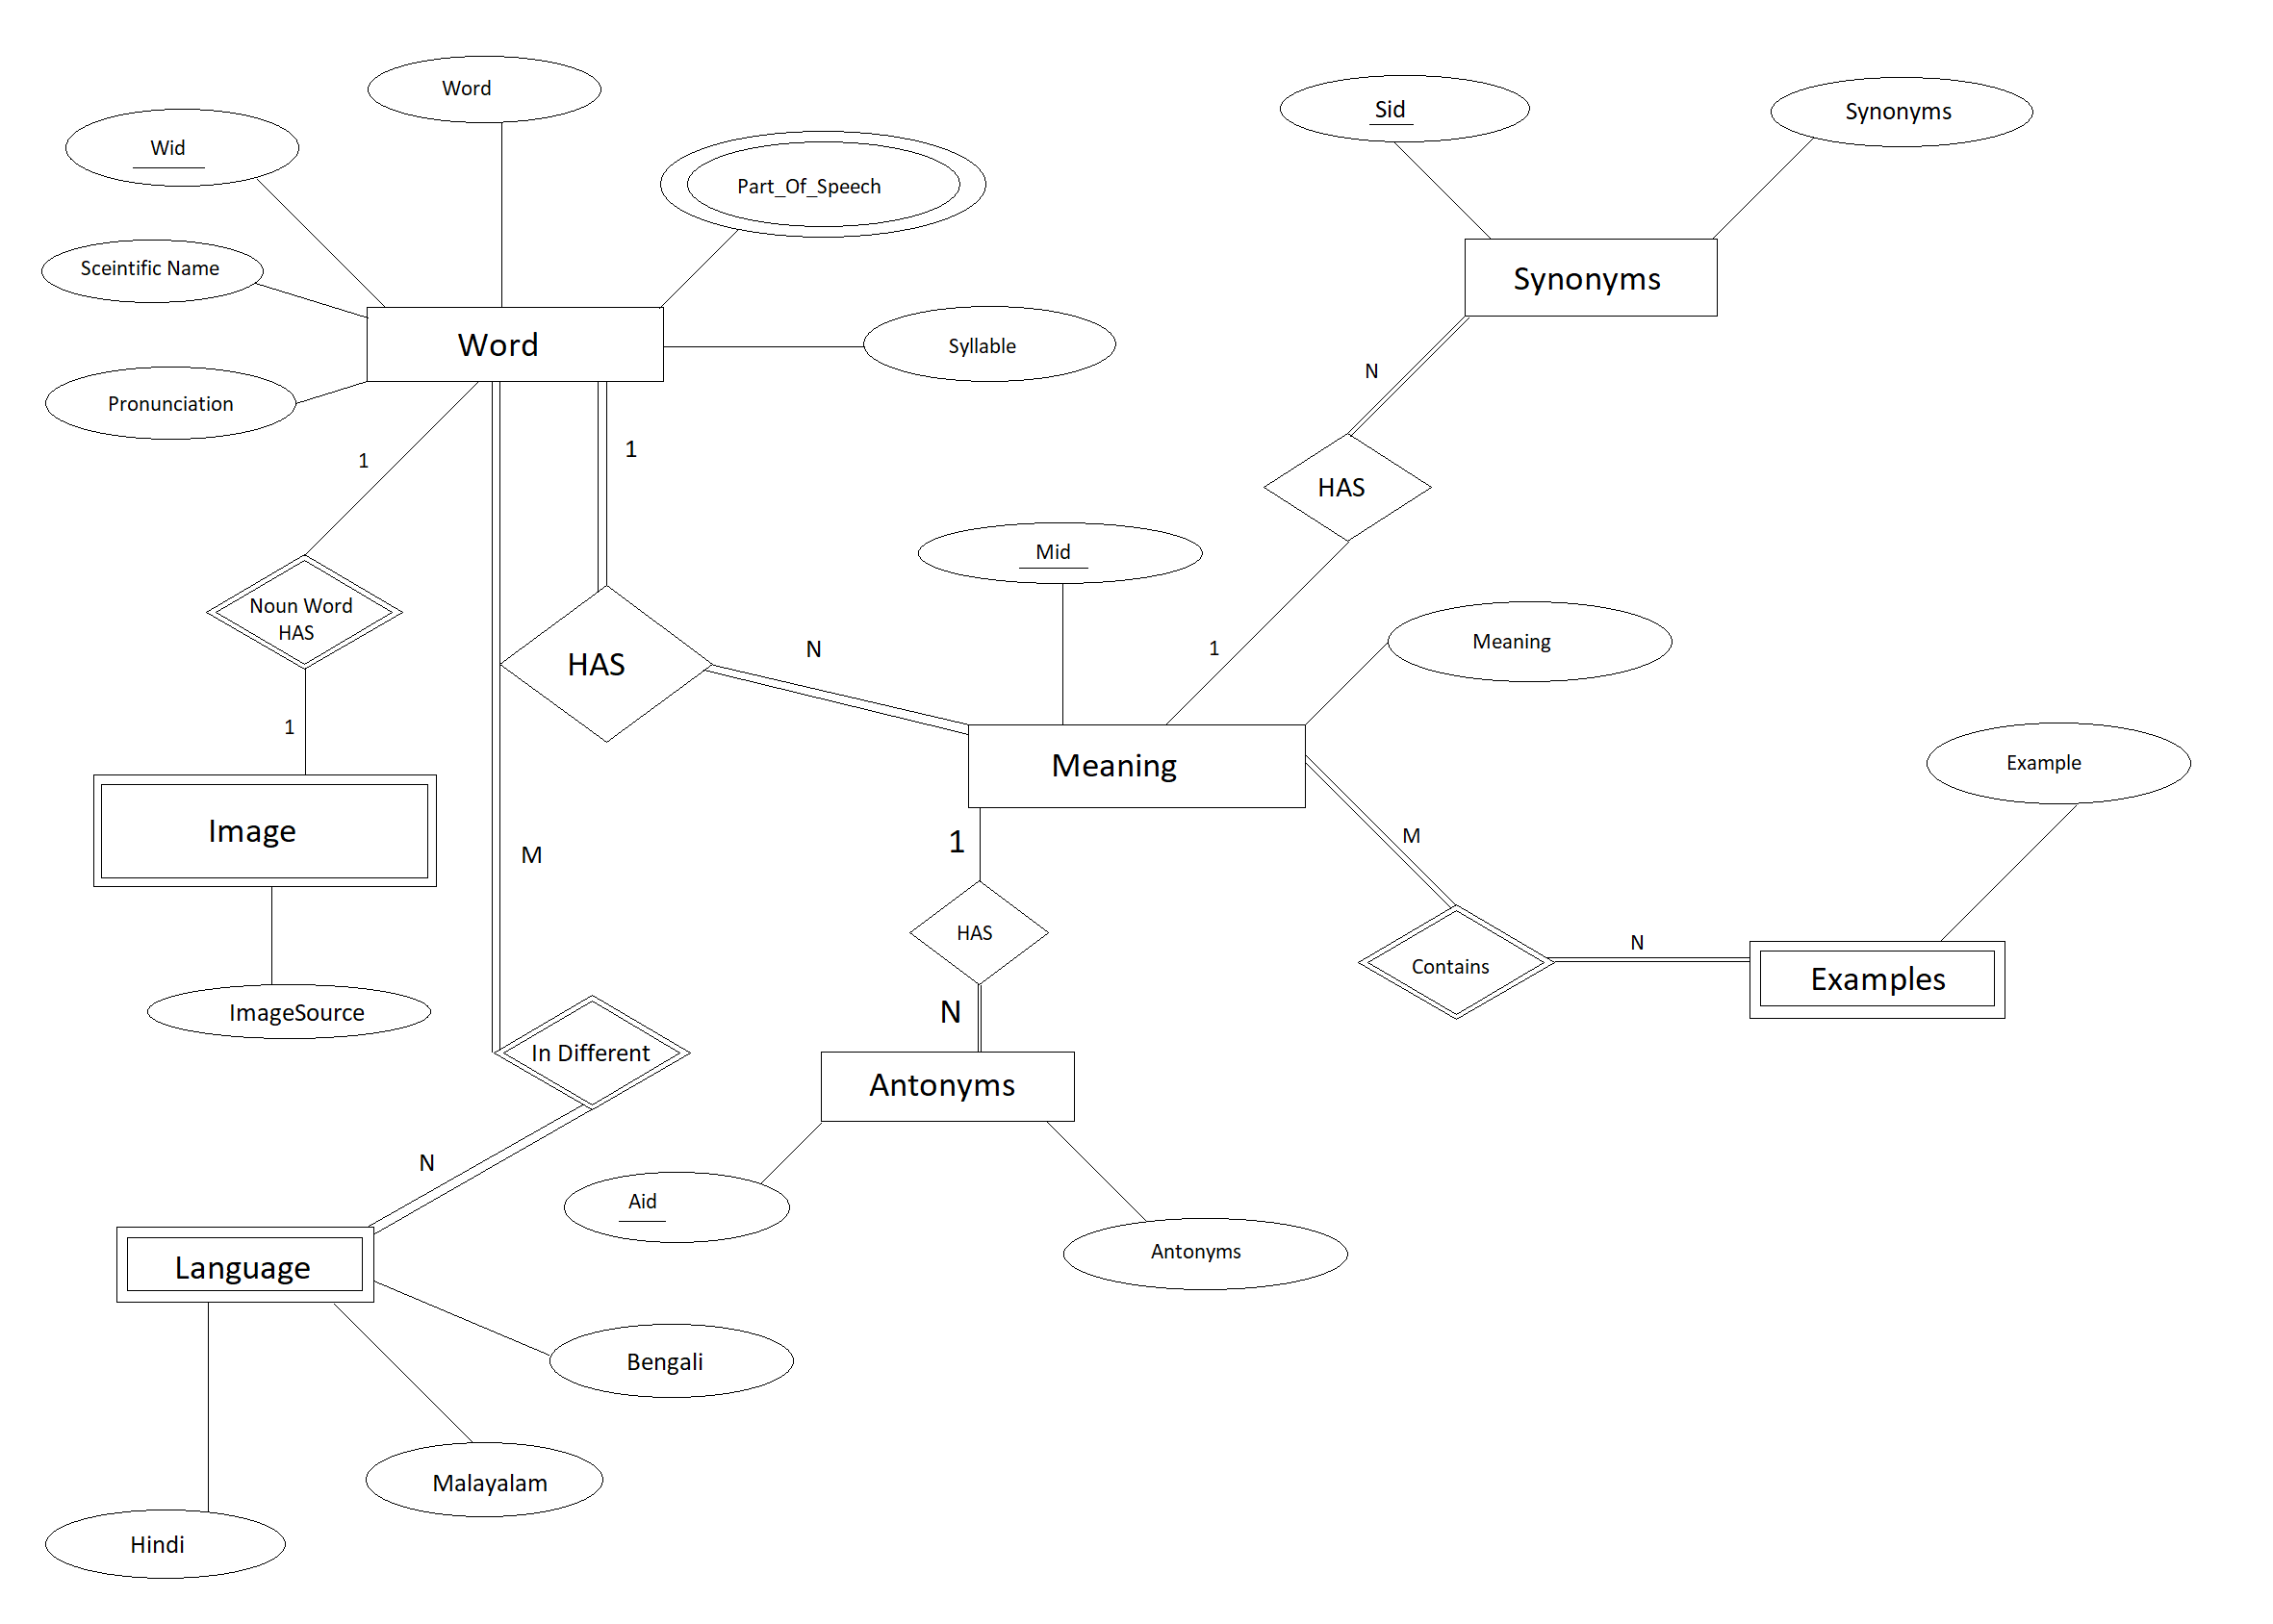
\includegraphics[width=1.3\textwidth]{ER_Diagram.png}
\end{center}
\pagebreak
\huge \textbf{Normalized Tables}\newline
\hline

\\
\subsection*{Word}
{\fontfamily{qcr}\selectfont

\begin{center}
\begin{tabular}{ |c|c| } 
 \hline
\large\underline{{Wid}} & \large{Word }\\  
 \hline
\end{tabular}
\end{center}
\newline
}

\subsection*{Syllable}
{\fontfamily{qcr}\selectfont

\begin{center}
\begin{tabular}{ |c|c| } 
 \hline
\large\underline{{Wid(FK)}} & \large{Syllable}\\  
 \hline
\end{tabular}
\end{center}
}

\subsection*{Pronunciation}
{\fontfamily{qcr}\selectfont

\begin{center}
\begin{tabular}{ |c|c| } 
 \hline
\large\underline{{Wid(FK)}} & \large{Pronunciation}\\  
 \hline
\end{tabular}
\end{center}
}

\subsection*{Meaning}
{\fontfamily{qcr}\selectfont

\begin{center}
\begin{tabular}{ |c|c|c|c| } 
 \hline
\large\underline{{Wid(FK)}} & \large\underline{{Pid(FK)}} & \large\underline{{Mid}} &\large{Meaning}\\  
 \hline
\end{tabular}
\end{center}
}

\subsection*{PartsOfSpeech}
{\fontfamily{qcr}\selectfont

\begin{center}
\begin{tabular}{ |c|c|c| } 
 \hline
\large\underline{{Pid(PK)}} & \large\underline{{Wid(FK)}} & \large{Part Of Speech}\\  
 \hline
\end{tabular}
\end{center}
}

\subsection*{Language}
{\fontfamily{qcr}\selectfont
\begin{center}
\begin{tabular}{ |c|c|c|c| } 
 \hline
\large\underline{{Wid(FK)}} & \large{Hindi} & \large{Malayalam} & \large{Bangla}\\  
 \hline
\end{tabular}
\end{center}
}

\subsection*{Image\large(Word Image)}
{\fontfamily{qcr}\selectfont
\begin{center}
\begin{tabular}{ |c|c|c| } 
 \hline
\large\underline{{Wid(FK)}} & \large\underline{{Pid(FK)}} & \large{ImageSource}\\  
 \hline
\end{tabular}
\end{center}
}

\subsection*{Sname\large(SientificName)}
{\fontfamily{qcr}\selectfont
\begin{center}
\begin{tabular}{ |c|c| } 
 \hline
\large\underline{{Wid(FK)}} &  \large{Scientific\textunderscore Name\\  
 \hline
\end{tabular}
\end{center}
}

\subsection*{Meaning\textunderscore Synonym}
{\fontfamily{qcr}\selectfont

\begin{center}
\begin{tabular}{ |c|c|c|c| } 
 \hline
\large\underline{{Pid(FK)}} & \large\underline{{Mid(FK)}} & \large\underline{{Sid}} &\large{Synonyms}\\  
 \hline
\end{tabular}
\end{center}
}

\subsection*{Meaning\textunderscore Antonym}
{\fontfamily{qcr}\selectfont
\begin{center}
\begin{tabular}{ |c|c|c|c| } 
 \hline
\large\underline{{Pid(FK)}} & \large\underline{{Mid(FK)}} & \large\underline{{Aid}} &\large{Antonyms}\\  
 \hline
\end{tabular}
\end{center}
}

\subsection*{Meaning\textunderscore Example}
{\fontfamily{qcr}\selectfont
\begin{center}
\begin{tabular}{ |c|c|c|} 
 \hline
\large\underline{{Pid(FK)}} & \large\underline{{Mid(FK)}} & \large{Example}\\  
 \hline
\end{tabular}
\end{center}
}
\pagebreak

\huge{Data Dictionary}\\ 
\hline

\subsection*{Word}
\begin{center}
\begin{tabular}{ |m{2em}|m{2em}|m{2em}|m{4cm}|m{2cm}| } 
 \hline
\large\textbf{Field Name} & \large\textbf{Data Type} & \large\textbf{Field Size} & \large\textbf{Description} & \large\textbf{Example}\\  
 \hline
\small Wid & \small Integer &\small 4 &\small Unique Id attached to each word as Primary Key &\small 8 \\
\hline
\small Word & \small varchar &\small 30 &\small Name of the Word &\small Articulate \\
\hline
\end{tabular}
\end{center}

\subsection*{Syllable}
\begin{center}
\begin{tabular}{ |m{2em}|m{2em}|m{2em}|m{4cm}|m{2cm}| } 
 \hline
\large\textbf{Field Name} & \large\textbf{Data Type} & \large\textbf{Field Size} & \large\textbf{Description} & \large\textbf{Example}\\  
 \hline
\small Wid & \small Integer &\small 4 &\small Foreign Key to the table referencing to the Primary Key of Word table &\small 4 \\
\hline
\small Syllable & \small varchar &\small 30 &\small Syllable of the Word &\small ar-tic-u-late \\
\hline
\end{tabular}
\end{center}

\pagebreak
\subsection*{Meaning}
\begin{center}
\begin{tabular}{ |m{2em}|m{2em}|m{2em}|m{7cm}|m{2cm}| } 
 \hline
\large\textbf{Field Name} & \large\textbf{Data Type} & \large\textbf{Field Size} & \large\textbf{Description} & \large\textbf{Example}\\  
 \hline
\small Wid & \small Integer &\small 4 &\small Foreign Key to the table referencing to the Primary Key of Word table &\small 7    \\
\hline
\small Pid & \small Integer &\small 4 &\small Foreign Key to the table referencing to the Primary Key of PartsOfSpeech table &\small 3 \\
\hline
\small Mid & \small Integer &\small 4 &\small Unique Id attached to each meaning as Primary Key combined with other Foreign Keys &\small 6 \\ 
\hline
\small Meaning & \small varchar &\small 200 &\small Meaning of the Word as per the part of speech of the word &\small Expressing yourself easily or characterized by clear expressive language \\
\hline
\end{tabular}
\end{center}

\subsection*{Parts Of Speech}
\begin{center}
\begin{tabular}{ |m{2em}|m{2em}|m{2em}|m{7cm}|m{2cm}| } 
 \hline
\large\textbf{Field Name} & \large\textbf{Data Type} & \large\textbf{Field Size} & \large\textbf{Description} & \large\textbf{Example}\\  
 \hline
\small Pid & \small Integer &\small 4 &\small Unique Id attached to each meaning as Primary Key combined with other Foreign Key &\small 6 \\
\hline
\small Wid & \small Integer &\small 4 &\small Foreign Key to the table referencing to the Primary Key of Word table &\small 1 \\
\hline
\small PartOfSpeech & \small varchar &\small 30 &\small Part of Speech of a word mapped with Pid and Wid &\small Adjective \\
\hline
\end{tabular}
\end{center}
\pagebreak

\subsection*{Pronunciation}
\begin{center}
\begin{tabular}{ |m{3em}|m{2em}|m{2em}|m{4cm}|m{2cm}| } 
 \hline
\large\textbf{Field Name} & \large\textbf{Data Type} & \large\textbf{Field Size} & \large\textbf{Description} & \large\textbf{Example}\\  
 \hline
\small Wid & \small Integer &\small 4 &\small Foreign Key to the table referencing to the Primary Key of Word table &\small 4 \\
\hline
\small Pronunciation & \small varchar &\small 30 &\small IPA Pronunciation of the word &\small 'dri$\eta$k} \\
\hline
\end{tabular}
\end{center}

\subsection*{Sname (Scientific Name)}
\begin{center}
\begin{tabular}{ |m{3.2em}|m{2em}|m{2em}|m{4cm}|m{2.2cm}| } 
 \hline
\large\textbf{Field Name} & \large\textbf{Data Type} & \large\textbf{Field Size} & \large\textbf{Description} & \large\textbf{Example}\\  
 \hline
\small Wid & \small Integer &\small 4 &\small Foreign Key to the table referencing to the Primary Key of Word table &\small 4 \\
\hline
\small Scientific\textunderscore Name & \small varchar &\small 50 &\small Scientific name of the living entities such as Flora and Fauna  &\small Earthworm is Lumbricina \\
\hline
\end{tabular}
\end{center}

\pagebreak
\subsection*{Image}
\begin{center}
\begin{tabular}{ |m{3em}|m{2em}|m{2.5em}|m{4cm}|m{2cm}| } 
 \hline
\large\textbf{Field Name} & \large\textbf{Data Type} & \large\textbf{Field Size} & \large\textbf{Description} & \large\textbf{Example}\\  
 \hline
\small Wid & \small Integer &\small 4 &\small Foreign Key to the table referencing to the Primary Key of Word table &\small 4 \\
\hline
\small Pid & \small Integer &\small 4 &\small Foreign Key to the table referencing to the Primary Key of PartsOfSpeech table &\small 2 \\
\hline
\small ImageSource & \small longblob &\small from 0 to 429467295 bytes &\small Image File of the records of Sname table  &\small  \\
\hline
\end{tabular}
\end{center}

\subsection*{Synonym}
\begin{center}
\begin{tabular}{ |m{3em}|m{2em}|m{2.5em}|m{4cm}|m{2cm}| } 
 \hline
\large\textbf{Field Name} & \large\textbf{Data Type} & \large\textbf{Field Size} & \large\textbf{Description} & \large\textbf{Example}\\  
 \hline
\small Pid & \small Integer &\small 4 &\small Foreign Key to the table referencing to the Primary Key of PartsOfSpeech table &\small 4 \\
\hline
\small Mid & \small Integer &\small 4 &\small Foreign Key to the table referencing to the Primary Key of Meaning table &\small 2 \\
\hline
\small Sid & \small Integer &\small 4 &\small Unique Id attached to each word as Primay Key &\small 9 \\
\hline
\small Synonym & \small varchar &\small 150 &\small Contains the Synonyms of the words  &\small Boastful has braggy, crowing, etc.  \\
\hline
\end{tabular}
\end{center}

\pagebreak

\subsection*{Antonym}
\begin{center}
\begin{tabular}{ |m{3em}|m{3em}|m{2em}|m{5cm}|m{2.2cm}| } 
 \hline
\large\textbf{Field Name} & \large\textbf{Data Type} & \large\textbf{Field Size} & \large\textbf{Description} & \large\textbf{Example}\\  
 \hline
\small Pid & \small Integer &\small 4 &\small Foreign Key to the table referencing to the Primary Key of PartsOfSpeech table &\small 4 \\
\hline
\small Mid & \small Integer &\small 4 &\small Foreign Key to the table referencing to the Primary Key of Meaning table &\small 2 \\
\hline
\small Aid & \small Integer &\small 4 &\small Unique Id attached to each word as Primay Key &\small 9 \\
\hline
\small Antonym & \small varchar &\small 50 &\small Contains the Antonyms of the words  &\small Boastful has humble  \\
\hline
\end{tabular}
\end{center}

\subsection*{Example}
\begin{center}
\begin{tabular}{ |m{3em}|m{3em}|m{2em}|m{5cm}|m{2.2cm}| } 
 \hline
\large\textbf{Field Name} & \large\textbf{Data Type} & \large\textbf{Field Size} & \large\textbf{Description} & \large\textbf{Example}\\  
 \hline
\small Pid & \small Integer &\small 4 &\small Foreign Key to the table referencing to the Primary Key of PartsOfSpeech table &\small 4 \\
\hline
\small Mid & \small Integer &\small 4 &\small Foreign Key to the table referencing to the Primary Key of Meaning table &\small 4 \\
\hline
\small Example & \small varchar &\small 200 &\small Example of a word w.r.t to its part of speech and meaning &\small I do not say that in any boastful spirit. \\
\hline
\end{tabular}
\end{center}

\pagebreak

\subsection*{Language}
\begin{center}
\begin{tabular}{ |m{3em}|m{2em}|m{2em}|m{3.8cm}|m{4cm}| } 
 \hline
\large\textbf{Field Name} & \large\textbf{Data Type} & \large\textbf{Field Size} & \large\textbf{Description} & \large\textbf{Example}\\  
 \hline
\small Wid & \small Integer &\small 4 &\small Foreign Key to the table referencing to the Primary Key of Word table &\small 4 \\
\hline

\small Hindi & \small varchar &\small 300 &\small Contains Hindi words of the searched English Word &\small Fragile: Hindi Words \\
\hline
\small Malayalam & \small varchar &\small 300 &\small Contains Malayalam words of the searched English Word &\small Fragile: Malayalam Words \\
\hline
\small Bengla & \small varchar &\small 300 &\small Contains Bengali words of the searched English Word &\small Fragile: Bengali Words \\
\hline
\end{tabular}
\end{center}

\pagebreak

\centering\huge{Words in Dictionary}\newline
\hline 
\begin{itemize}
    \large\item Articulate \\
    \large\item Artillery \\
    \large\item Boastful \\
    \large\item Coaxial \\
    \large\item Daemon \\
    \large\item Deadlock \\
    \large\item Earthworm \\
    \large\item Fabulous \\
    \large\item Fragile \\
    \large\item Giraffe \\
\end{itemize}

\pagebreak
\centering\huge{BIBLIOGRAPHY}\newline
\hline 

\begin{enumerate}
   \large\item Merriam Webster : \href{https://www.merriam-webster.com/}{}\\
   To search for the meaning of the words and synonyms in English. \\

   \large\item Cambridge Dictionary : \href{https://dictionary.cambridge.org/}{}\\
   To search for the meaning of the words and synonyms in English. \\

   \large\item Shabdkosh Hindi : \href{https://www.shabdkosh.com/dictionary/english-hindi/}{}\\
   To search the words, Hindi translation from English . \\

   \large\item Shabdkosh Malayalam : \href{https://www.shabdkosh.com/dictionary/english-malayalam/}{}\\
   To search the words, Malayalam translation from English . \\

   \large\item Shabdkosh Bengali : \href{https://www.shabdkosh.com/dictionary/english-bengali/}{}\\
   To search the words, Bengali translation from English . \\   
\end{enumerate}
\end{document}
